\documentclass[a4paper]{article}
\usepackage{dirtytalk}
\usepackage{graphicx}
\usepackage{xcolor}
\usepackage{url}
\usepackage{outlines}
\usepackage{listings}
\usepackage{fontspec}
% \setmainfont{Calibri}
\lstset{basicstyle=\ttfamily,
	showstringspaces=false,
	commentstyle=\color{blue},
	keywordstyle=\color{pink}
}
\lstset{emph={
	nc,tcp,udp,http,},emphstyle=\color{purple}
}
\usepackage{fancyhdr}
\usepackage{geometry}
\geometry{
	a4paper,
	total={170mm,257mm},
	left=20mm,
	top=20mm,
	bottom=39mm,
}
\newcommand{\abc}{\hfill \break}
\setlength{\headheight}{82.70538pt}

\fancypagestyle{oida}{
	\fancyhf{}
	\fancyhead[L]{\fontsize{7.5}{7.5}htl donaustadt\\ Donaustadtstraße 45\\
		1220 Wien\\~\\ Abteilung: Informationstechnologie\\ 
	Schwerpunkt: Netzwerktechnik}
	\fancyhead[R]{
\includegraphics[scale=0.45]{images/logo.png}}

	\fancyfoot[L]{\today}
	\fancyfoot[C]{\jobname}
	\fancyfoot[R]{Seite: \thepage}
}

\begin{document}
\bibliographystyle{plain}
\pagestyle{oida}
\section*{Thema}
\par\noindent\rule{\textwidth}{0.4pt}

Laborprotokoll
Template

\begin{figure}[h]
	
\includegraphics[scale=0.3]{images/mika.jpeg}
	\caption{Wunderbares Gruppenlogo}
\end{figure}

\vspace*{\fill}
Unterrichtsgegenstand:	NWT|ANGE/ZIVK

Jahrgang:	3AHITN

Name:	Stefan Fürst, Marcel Raichle

Gruppenname/Nummer: Dumm und Dümmer/7

Betreuer: 	ANGE,ZIVK

Übungsdaten:	18.10.2024, 25.10.2024

Abgabedatum:	7.11.2024


\newpage
\tableofcontents

\newpage

\section{Aufgabenstellung}

Grundlegende Konfiguration eines Switches, Verwaltung der Mac-Adresstabelle und Einrichtung eines SSH-Servers.


\section{Zusammenfassung}
Bei diesem Versuch wird ein Cisco-Switch auf minimale Konfiguration eingestellt, die MAC-Anschriftstabelle verwaltet und ein SSH-Server für Fernverwaltung eingerichtet. Als Nächstes überprüfen wir die Standardkonfiguration des Switches und konfigurieren die grundlegendsten Einstellungen einschließlich des Hostnamens, der Passwörter und eines MOTD-Banner. VLAN 99 wird für das Management eingerichtet, und eine statische IP-Adresse wird zugewiesen. Wir definieren ein Standard-Gateway, um auf den Switch zugreifen zu können, und überprüfen die Konnektivität mithilfe von Ping-Tests. Darüber hinaus verwalten wir die MAC-Anschriftstabelle, indem dynamische und statische MAC-Anschriften angezeigt und konfiguriert werden. Abschließend wird ein SSH-Server konfiguriert, um das sichere Fernen des Geräts zu ermöglichen.
\newpage

\section{Vollständige Netzwerktopologie der gesamten Übung}

\begin{figure}[h]
	\centering
	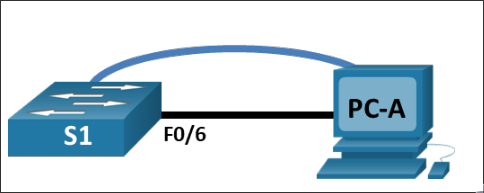
\includegraphics[scale=1.5]{images/asfadsopfosdf.png}
	\caption{Vollständige Netzwerktopologie der gesamten Übung}
\end{figure}

\newpage

\section{Übungsdurchführung}
%überschriften auf deutsch übersetzen
\subsection{Verkabeln Sie den Nework und überprüfen Sie die Standard-Switch-Konfiguration}
\subsubsection{Verkabeln Sie das Netz wie in der Topologie dargestellt.} 
\paragraph{1a}\abc
Das SDM-Bias-Template bietet keine IPv6-Adressfunktionen. Um sicherzustellen, dass der SDM das Dual-IPv4- und IPv6-Template oder das Lanbase-Routing-Template verwendet, müssen die folgenden Befehle verwendet werden.
\begin{lstlisting}
Switch# configure terminal
Switch(config)# sdm prefer dual-ipv4-and-ipv6 default
Switch(config)# end
Switch# reload
\end{lstlisting}
\paragraph{1b} \abc
\begin{itemize}
	\item \say {Warum müssen Sie für die Erstkonfiguration des Switches eine Konsolenverbindung verwenden? Warum ist es nicht möglich, sich über Telnet oder SSH mit dem Switch zu verbinden?} \abc
\begin{itemize}
	\item Standardmäßig hat der Switch keine Netzwerkkonfiguration.
\end{itemize}
\end{itemize}
\subsubsection{Überprüfen Sie die Standardkonfiguration des Switches.}
\paragraph{2b} \abc
\begin{itemize}
\item \say{Wie viele FastEthernet-Schnittstellen hat ein 2960-Switch?} \abc
\begin{itemize}
\item Der Cisco 2960 hat 24 FastEthernet-Schnittstellen.\abc
\end{itemize}
\item \say{Wie viele GigabitEthernet-Schnittstellen hat ein 2960-Switch?} \abc
\begin{itemize}
\item Der Cisco 2960 hat 2 GiagibtEthernet-Schnittstellen.\abc
\end{itemize}
\item \say{Welcher Wertebereich wird für die vty-Lines angezeigt?} \abc
\begin{itemize}
\item Es wird der Wertebereich 5-15 angezeigt. \abc
\end{itemize}
\end{itemize}
\paragraph{2c} \abc
\begin{lstlisting}
Switch# show startup-config
startup-config is not present
\end{lstlisting}
Dies bedeutet, dass keine Startkonfiguration im NVRAM gespeichert wurde.
\paragraph{2d} \abc
Um die Eigenschaften des SVI in VLAN1 anzuzeigen, wird der folgende Befehl verwendet \texttt{show ip interface vlan1}. \abc
In VLAN1 ist standardmäßig keine IP-Adresse vorhanden. \abc
Die MAC-Adresse des SVI wird mit dem Befehl \texttt{mac addr} angezeigt und lautet in diesem Fall \texttt{0018.18bc.59c0}. \abc
VLAN1 ist administratively down, line protocol is down bis eine Schnittstelle in Betrieb genommen wird. \abc
\paragraph{2e} \abc
Um die IP-Eigenschaften der SVI von VLAN1 anzuzeigen, wird der Befehl \texttt{show ip interface vlan1} verwendet, der folgende Ausgabe erzeugt: 
\begin{lstlisting}
Vlan1 is administratively down, line protocol is down
Internet protocol processing disabled	
\end{lstlisting}
\paragraph{2f} \abc
\begin{lstlisting}
Switch# show ip interface vlan1
Vlan1 is administratively up, line protocol is up
Internet protocol processing disabled	
\end{lstlisting}
Jetzt ist der Status auf up, da ein Host mit einer Schnittstelle verbunden wurde. Deshalb ist jetzt auch VLAN1 up, da standardmäßig alle Schnittstellen in VLAN1 sind.
\paragraph{2g} \abc
Informationen über das Gerät können mit \texttt{show version} ausgegeben werden. \abc
Hier kann man die Version ablesen, die in diesem Fall 12.12 ist, und die Base MAC Adresse, die \texttt{00:18:18:BC:59:80} ist. \abc
Mit \texttt{show flash} wird der Dateiname des geladenen Images angezeigt, in diesem Fall \texttt{c3560-ipservicesk9-mz.122-55.SE6.bin}. \abc
\paragraph{2h} \abc
Informationen über die Schnittstelle, an die der Host angeschlossen ist, werden mit \texttt{show interface f0/6} angezeigt.\abc
Die Schnittstelle ist up, da ein Gerät angeschlossen ist, die MAC-Adresse ist \texttt{0018.18bc.5988} und die Duplex-Einstellungen sind \texttt{Full-duplex, 100Mb/s,}. \abc
\paragraph{2i} \abc
Mit \texttt{show vlan} können Informationen über VLANs auf dem Switch angezeigt werden. \abc
\paragraph{2j} \abc
Mit \texttt{show flash} oder \texttt{dir flash} kann der Inhalt des Flash-Verzeichnisses, in diesem Fall \texttt{c3560-ipservicesk9-mz.122-55.SE6.bin}, angezeigt werden. \abc
Die \texttt{.bin} Datei ist das Image, von dem der Switch bootet und auch die einzige Datei in diesem Verzeichnis.
\subsection{Basis Netzwerk Konfiguration des Switches}
\subsubsection{Basiseinstellungen des Switches}
\paragraph {1a} \abc
Folgende Befehle einfügen:
\begin{lstlisting}
no ip domain-lookup
hostname S1
service password-encryption
enable secret class
banner motd #
Unauthorized access is strictly prohibited. #
\end{lstlisting}
\paragraph {1b} \abc
Bevor der Switch über das Netzwerk verwaltet werden kann, muss ihm eine IP-Adresse zugewiesen werden, aber bevor dies geschieht, wird das Management-VLAN von VLAN1 auf ein anderes VLAN, in diesem Fall 99, geändert.
\begin{lstlisting}
S1# conf t
S1(config)# vlan 99 
S1(config-vlan)# exit
S1(config)# interface vlan99
S1(config-if)# ip address 192.168.1.2 255.255.255.0
S1(config-if)# ipv6 address 2001:db8:acad::2/64
S1(config-if)# ipv6 address fe80::2 link-local
S1(config-if)# no shutdown
\end{lstlisting}
\paragraph {1c} \abc
Die folgenden Befehle werden verwendet, um alle Schnittstellen in VLAN99 zuzuweisen:
\begin{lstlisting}
S1(config)# interface range f0/1 – 24,g0/1 - 2
S1(config-if-range)# switchport access vlan 99
S1(config-if-range)# exit
\end{lstlisting}
d
\paragraph {1d} \abc
Mit \texttt{show vlan brief} werden die zuvor zugewiesenen Schnittstellen angezeigt.
\begin{figure}[h]
	\centering
	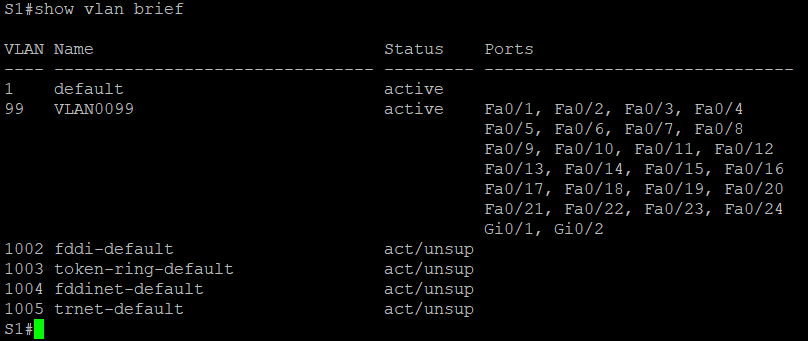
\includegraphics[scale=0.4]{images/show-vlan-brief.png}
	\caption{show vlan brief}
\end{figure}
\paragraph {1e} \abc
Wenn kein Standardgateway konfiguriert ist, kann der Switch nicht über das Netzwerk verwaltet werden und muss daher mit dem Befehl \texttt{ip default-gateway 192.168.1.1} konfiguriert werden.
\paragraph {1f} \abc
Um den Konsolenzugang mit einem Passwort zu sichern, wird die \texttt{line 0} (Konsolenzugang) konfiguriert und mit dem Befehl \texttt{password} ein Passwort gesetzt.
\begin{lstlisting}
S1(config)# line con 0
S1(config-line)# logging synchronous
S1(config-line)# password cisco
S1(config-line)# login
S1(config-line)# exit
\end{lstlisting}
\paragraph {1g} \abc
Der Befehl \texttt{login} ist notwendig, da sonst kein Passwort abgefragt wird.

\subsubsection{Konfiguration der IP-Adresse des PC}\abc
Öffnen Sie dazu die Systemsteuerung, gehen Sie zu Netzwerk und Freigabecenter und tragen Sie unter Adaptereinstellungen bei ip4/6 die IP-Adressen aus der Tabelle ein.
\begin{figure}[h]
	\centering
	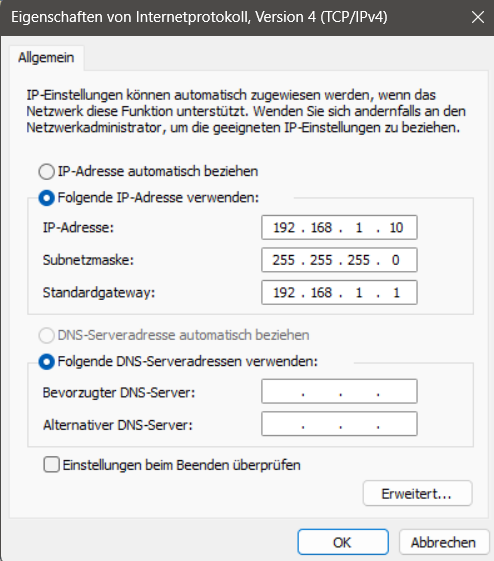
\includegraphics[scale=0.4]{images/ipv4.png}
	\caption{Konfiguration der IPv4-Adresse}
\end{figure}
\begin{figure}[h]
	\centering
	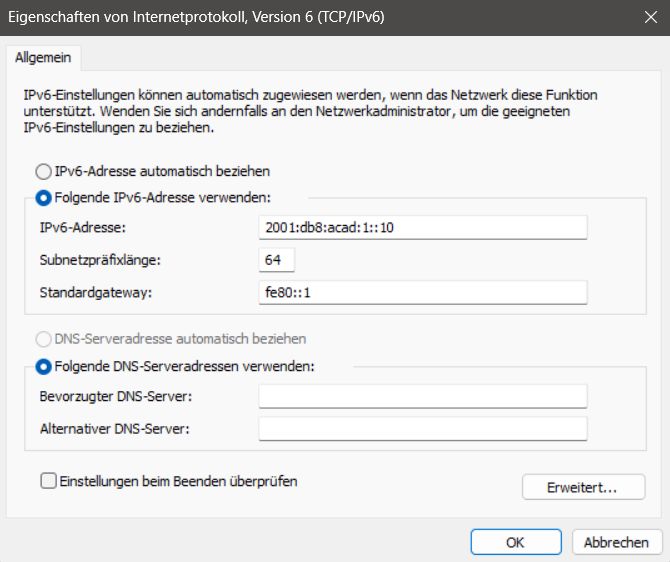
\includegraphics[scale=0.4]{images/ipv6.png}
	\caption{Konfiguration der IPv6-Adresse}
\end{figure}
\subsection{Verify and Test Network Connectivity} \abc
a
show run
\paragraph {1b} \abc
Um die Einstellungen von VLAN99 zu überprüfen, wird der Befehl \texttt{show interface vlan99} Befehl verwendet.
Hieraus geht hervor, dass die Bandbreite \texttt{1000000 Kbit} beträgt und der Status von VLAN99 und von line up ist.
\newpage
\subsubsection{Testen der Verbindung}\abc
Zum Testen der Verbindung wird das Programm \texttt{ping} verwendet.
\begin{figure}[h]
	\centering
	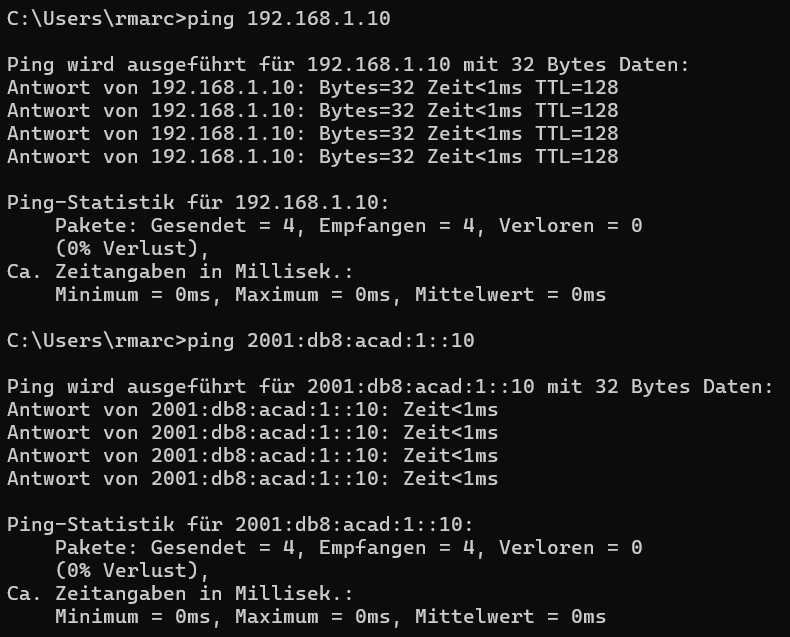
\includegraphics[scale=0.4]{images/ping.png}
	\caption{Ping zum SVIs des Swichts}
\end{figure}

\subsection{Verwalten der MAC-Adressen-Tabelle}
\subsubsection{Host-MAC-Adresse ermitteln}
Mit dem Befehl \texttt{getmac -v} können alle MAC-Adressen angezeigt werden.
\begin{figure}[h]
	\centering
	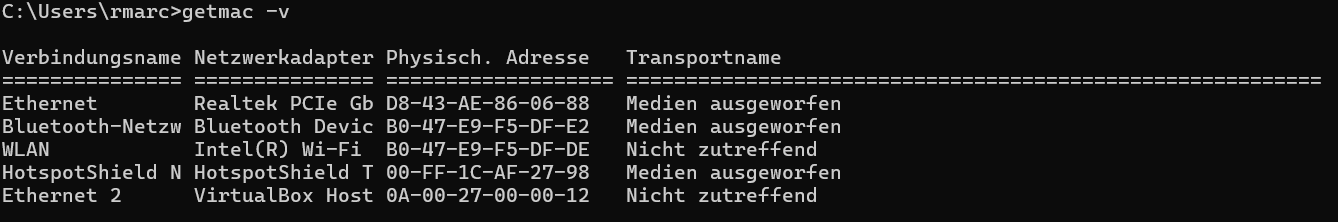
\includegraphics[scale=0.3]{images/getmac.png}
	\caption{getmac -v}
\end{figure}
Die MAC-Adresse der verwendeten Ethernet-Schnittstelle lautet \texttt{D8-43-AE-86-06-88}.

\newpage
\subsubsection{Ermitteln Sie die MAC-Adressen, die der Switch gelernt hat.}
Mit dem Befehl \texttt{show mac address-table} kann die MAc-Adresstabelle ausgegeben werden.\abc
\begin{figure}[h]
	\centering
	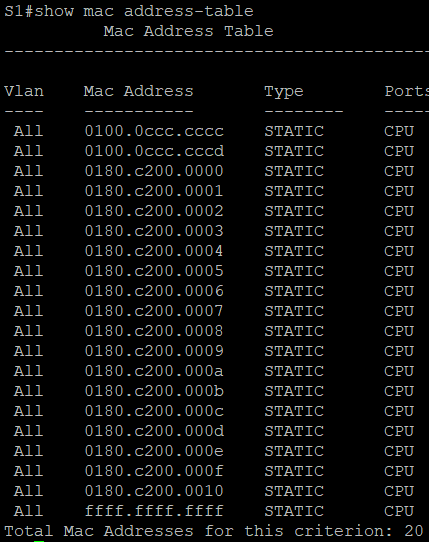
\includegraphics[scale=0.4]{images/show-mac-addr-table.png}
	\caption{show mac address-table}
\end{figure}\abc
Es werden 2 dynamische MAC-Adressen angezeigt und es gibt insgesamt 22 MAC-Adresseneinträge und die MAC-Adresse stimmt mit der des Hosts überein. \abc
\subsubsection{Anzeigen der show mac address-table Optionen}

\begin{figure}[h]
	\centering
	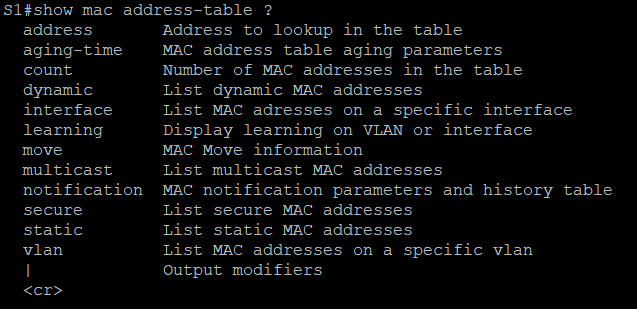
\includegraphics[scale=0.4]{images/show-table.otpion.png}
	\caption{show mac address-table ?}
\end{figure}\abc
\begin{figure}[h]
	\centering
	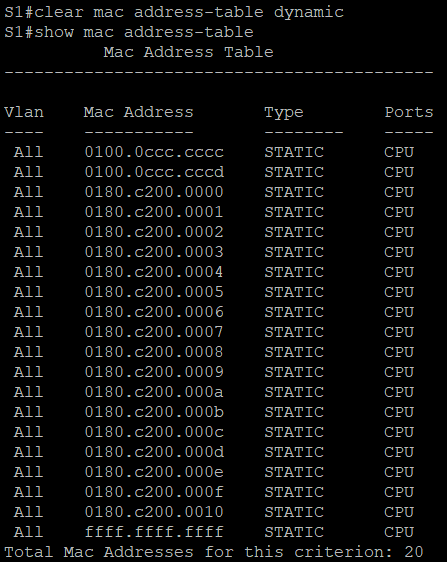
\includegraphics[scale=0.4]{images/dynamic.png}
	\caption{show mac address-table dynamic}
\end{figure}\abc
Es sind 13 dynamische MAC-Adressen eingetragen. \abc

Der Befehl \texttt {show mac address-table address D8-43-AE-86-06-88} zeigt nur den Host-Eintrag an.
\subsubsection{Einstellung der statischen Mac-Adressen}
Die dynamischen Mac-adresen werden aus der MAC-Adressentable mit \texttt{clear mac address-table dynamic} gelöscht.\abc
\begin{figure}[h]
	\centering
	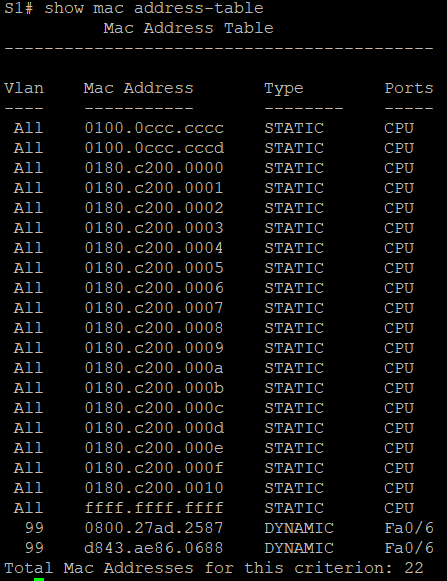
\includegraphics[scale=0.4]{images/uesdghdsughdsg.png}
	\caption{show mac-addres-table}
\end{figure}\abc
Es ist eine dynamische MAC-Adresse eingetragen, da der Switch diese dynamisch angefordert hat. \abc
Der Befehl \texttt{mac address-table static d843.ae86.0688 vlan 99 interface fastethernet 0/6} fügt die MAC-Adresse des Hosts als statischen Eintrag in die Tabelle ein, so dass es nun 22 statische Einträge in der Tabelle gibt.\abc
\begin{figure}[h]
	\centering
	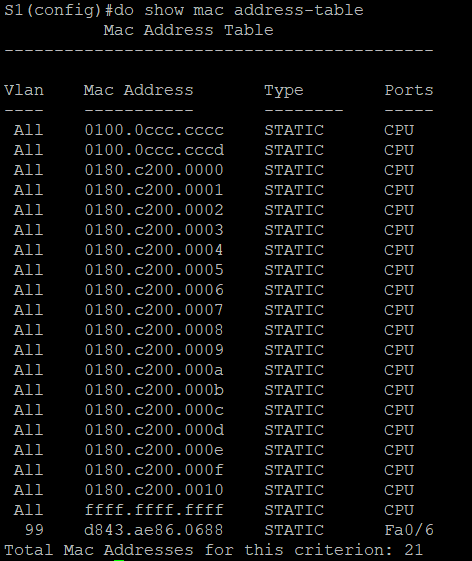
\includegraphics[scale=0.4]{images/thign.png}
	\caption{Nur statische Einträge}
\end{figure}\abc


Mit dem Befehl \texttt{no mac address-table static d843.ae86.0688 vlan 99 interface fastethernet 0/6} wird dieser Eintrag wieder entfernt, woraufhin die Tabelle wieder wie zuvor 20 statische Einträge enthält.

\begin{figure}[h]
	\centering
	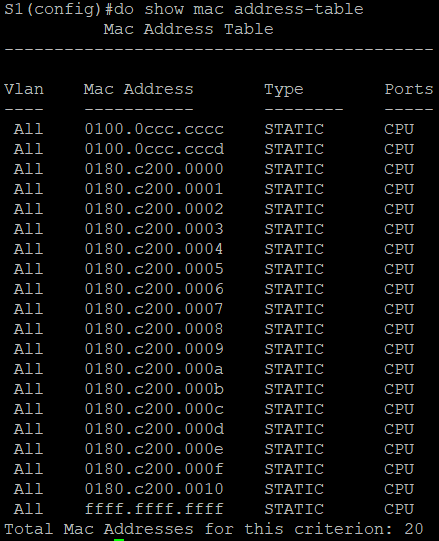
\includegraphics[scale=0.4]{images/macddr3.png}
	\caption{Wieder 20 statische Einträge}
\end{figure}\abc


\subsection{Reflection quenstions}
\begin{enumerate}
	\item Warum sollten Sie das vty-Passwort für den Switch konfigurieren?
\begin{enumerate}
	\item Wenn Sie kein vty-Passwort konfigurieren, können Sie nicht mit Telnet auf den Switch zugreifen.
\end{enumerate}
\item Warum sollte das Standard-VLAN 1 in eine andere VLAN-Nummer geändert werden?
\begin{enumerate}
	\item Für eine verbesserte Sicherheit.
\end{enumerate}
\item Wie kann man verhindern, dass Kennwörter im Klartext gesendet werden?
\begin{enumerate}
	\item Mit dem Befehl \texttt{service password-encryption} ein.
\end{enumerate}
\item Warum eine statische MAC-Adresse auf einer Port-Schnittstelle konfigurieren?
\begin{enumerate}
	\item So legen Sie fest, mit welchen Ports sich ein Host verbinden kann.
\end{enumerate}
\end{enumerate}



\newpage

\subsubsection{SSH}
\begin{lstlisting}
%Domänennamen festlegen
ip domain-name htl-donaustadt.at
%RSA-key generieren
crypto key gen rsa
benutzer anlegen
%secret statt password, damit das Passwort nicht in Klartext gespeichert wird.
username name secret cisco
%lokale Benutzerdatenbank benutzen und einschalten
login local
logging synchronous
%Vier gleichteige Verbindungen erlauben
line vty 0 4 4 weil 4 gleichzeitige verbindgen erlauben
login local
%ssh aktivieren
transport input ssh
%Abspeichern der Running-config in der startup-config
do wr
\end{lstlisting}
\newpage
\subsubsection{Switch Zurücksetzen nach der Übung}
\begin{lstlisting}
en
show flash
delete vlan.dat
enter drücken
erase startup-config
reload
no
\end{lstlisting}
\section{Vollständige Konfigurationsdateien}

\begin{lstlisting}
	
Current configuration : 3608 bytes
!
version 12.2
no service pad
service timestamps debug datetime msec
service timestamps log datetime msec
service password-encryption
!
hostname S1
!
boot-start-marker
boot-end-marker
!
enable secret 5 $1$WG/H$ILJURiwvDuU5JlSgXmVwY/
!
username name secret 5 $1$RrXg$grWbyFauxAuHdmwpC69tK.
!
no aaa new-model
system mtu routing 1500
no ip domain-lookup
ip domain-name htl-donaustadt.at
!
crypto pki trustpoint TP-self-signed-662526720
 enrollment selfsigned
 subject-name cn=IOS-Self-Signed-Certificate-662526720
 revocation-check none
 rsakeypair TP-self-signed-662526720
!
crypto pki certificate chain TP-self-signed-662526720
 certificate self-signed 01
  30820239 308201A2 A0030201 02020101 300D0609 2A864886 F70D0101 04050030
  30312E30 2C060355 04031325 494F532D 53656C66 2D536967 6E65642D 43657274
  69666963 6174652D 36363235 32363732 30301E17 0D393330 33303130 30303130
  345A170D 32303031 30313030 30303030 5A303031 2E302C06 03550403 1325494F
  532D5365 6C662D53 69676E65 642D4365 72746966 69636174 652D3636 32353236
  37323030 819F300D 06092A86 4886F70D 01010105 0003818D 00308189 02818100
  E8CE9436 BED8F37A A6DCE351 5227D20F B07A6BC0 FA0445B9 CEDC0064 57A2B496
  39161F3F D82FAB21 BA4D34D7 4DB51AAF 0A42E5C1 93AC51A4 B61D11F8 9CC33A19
  51920ADB 3266102A 8A5745DA 06ABA47C FECC8C07 AF90612C 412CB8E3 F26E329C
  CC17F9E2 81D47732 B02C8AC9 33C82388 87D3E4DF 2E86B505 E4170470 021733ED

S1\#sh run
Building configuration...

Current configuration : 3608 bytes
!
version 12.2
no service pad
service timestamps debug datetime msec
service timestamps log datetime msec
service password-encryption
!
hostname S1
!
boot-start-marker
boot-end-marker
!
enable secret 5 $1$WG/H$ILJURiwvDuU5JlSgXmVwY/
!
username name secret 5 $1$RrXg$grWbyFauxAuHdmwpC69tK.
!
no aaa new-model
system mtu routing 1500
no ip domain-lookup
ip domain-name htl-donaustadt.at
!
crypto pki trustpoint TP-self-signed-662526720
 enrollment selfsigned
 subject-name cn=IOS-Self-Signed-Certificate-662526720
 revocation-check none
 rsakeypair TP-self-signed-662526720
!
crypto pki certificate chain TP-self-signed-662526720
 certificate self-signed 01
  30820239 308201A2 A0030201 02020101 300D0609 2A864886 F70D0101 04050030
  30312E30 2C060355 04031325 494F532D 53656C66 2D536967 6E65642D 43657274
  69666963 6174652D 36363235 32363732 30301E17 0D393330 33303130 30303130
  345A170D 32303031 30313030 30303030 5A303031 2E302C06 03550403 1325494F
  532D5365 6C662D53 69676E65 642D4365 72746966 69636174 652D3636 32353236
  37323030 819F300D 06092A86 4886F70D 01010105 0003818D 00308189 02818100
  E8CE9436 BED8F37A A6DCE351 5227D20F B07A6BC0 FA0445B9 CEDC0064 57A2B496
  39161F3F D82FAB21 BA4D34D7 4DB51AAF 0A42E5C1 93AC51A4 B61D11F8 9CC33A19
  51920ADB 3266102A 8A5745DA 06ABA47C FECC8C07 AF90612C 412CB8E3 F26E329C
  CC17F9E2 81D47732 B02C8AC9 33C82388 87D3E4DF 2E86B505 E4170470 021733ED
  02030100 01A36330 61300F06 03551D13 0101FF04 05300301 01FF300E 0603551D
  11040730 05820353 312E301F 0603551D 23041830 16801460 47280E51 C2029C61
  DF3F8BB8 D9255894 39459730 1D060355 1D0E0416 04146047 280E51C2 029C61DF
  3F8BB8D9 25589439 4597300D 06092A86 4886F70D 01010405 00038181 00C0E85C
  A8F3A3E8 D613AA85 A036A6F4 3A1DD66B F05114A6 D03A2A06 620A9D2D 460E0F53
  B94F1B4F DE21ECDD BBD7C1D1 1A3C17B9 BAE76D91 C08AF26C FEBBBF0A 05A2653F
  596632F5 38D8C1C6 0C5A58F3 C90C797E 99E9E3AC 48AA92A4 F2F59711 6987BBA3
  A761D3BA AE41B89F 6933C814 87608BAD C087AB4C E681B888 73A5BE20 6E
  quit
!
spanning-tree mode pvst
spanning-tree extend system-id
!
vlan internal allocation policy ascending
!
interface FastEthernet0/1
 switchport access vlan 99
!
interface FastEthernet0/2
 switchport access vlan 99
!
interface FastEthernet0/3
 switchport access vlan 99
!
interface FastEthernet0/4
 switchport access vlan 99
!
interface FastEthernet0/5
 switchport access vlan 99
!
interface FastEthernet0/6
 switchport access vlan 99
!
interface FastEthernet0/7
 switchport access vlan 99
!
interface FastEthernet0/8
 switchport access vlan 99
!
interface FastEthernet0/9
 switchport access vlan 99
!
interface FastEthernet0/10
 switchport access vlan 99
!
interface FastEthernet0/11
 switchport access vlan 99
!
interface FastEthernet0/12
 switchport access vlan 99
!
interface FastEthernet0/13
 switchport access vlan 99
!
interface FastEthernet0/14
 switchport access vlan 99
!
interface FastEthernet0/15
 switchport access vlan 99
!
interface FastEthernet0/16
 switchport access vlan 99
!
interface FastEthernet0/17
 switchport access vlan 99
!
interface FastEthernet0/18
 switchport access vlan 99
!
interface FastEthernet0/19
!
interface FastEthernet0/20
!
interface FastEthernet0/21
!
interface FastEthernet0/22
!
interface FastEthernet0/23
!
interface FastEthernet0/24
!
interface GigabitEthernet0/1
!
interface GigabitEthernet0/2
!
interface Vlan1
 no ip address
 shutdown
!
interface Vlan99
 ip address 10.0.0.69 255.255.255.0
!
ip classless
ip http server
ip http secure-server
!
line con 0
line vty 0 4
 login local
 transport input ssh
line vty 5 15
 login
!
end
\end{lstlisting}
\newpage

\section{Quellen}
\bibliography{quellen}
\newpage
\section{Abbildungsverzeichnis}

\listoffigures

\end{document}
